\documentclass[12pt, a4paper]{report}
%\documentclass[11pt, a4paper]{article}

%====================== PACKAGES ======================
\usepackage[french]{babel}

\frenchbsetup{StandardLists=true}
\usepackage{enumitem}
\usepackage{pifont}

\usepackage[utf8x]{inputenc}
%\usepackage[latin1]{inputenc}

%pour gérer les positionnement d'images
\usepackage{float}
\usepackage{amsmath}
\DeclareMathOperator{\dt}{dt}
\usepackage{amsfonts}
\usepackage{graphicx}
\usepackage[colorinlistoftodos]{todonotes}
\usepackage{url}

%pour les informations sur un document compilé en PDF et les liens externes / internes
\usepackage[pdfborder=0]{hyperref}
\hypersetup{
	colorlinks = true
	}

%pour la mise en page des tableaux
\usepackage{array}
\usepackage{tabularx}
\usepackage{multirow}
\usepackage{multicol}
\setlength{\columnsep}{50pt}

%pour utiliser \floatbarrier
%\usepackage{placeins}
%\usepackage{floatrow}

%espacement entre les lignes
\usepackage{setspace}

%modifier la mise en page de l'abstract
\usepackage{abstract}

%police et mise en page (marges) du document
\usepackage[T1]{fontenc}
\usepackage[top=2cm, bottom=2cm, left=2cm, right=2cm]{geometry}

%Pour les galerie d'images
\usepackage{subfig}

\usepackage{pdfpages}

\usepackage{tikz}
\usetikzlibrary{trees}
\usetikzlibrary{decorations.pathmorphing}
\usetikzlibrary{decorations.markings}
\usetikzlibrary{decorations.pathreplacing,calligraphy}
\usetikzlibrary{decorations.pathmorphing,calc,shapes,shapes.geometric,patterns}
\usetikzlibrary{calc,intersections}
%\usetikzlibrary{decorations}
\usetikzlibrary{angles, quotes}
\usepackage{verbatim}

\usepackage{appendix}

\usepackage{comment}

\usepackage{xcolor}

%\PreviewEnvironment{tikzpicture}
%\setlength\PreviewBorder{0pt}%

%====================== INFORMATION ET REGLES ======================

%rajouter les numérotation pour les \paragraphe et \subparagraphe
\setcounter{secnumdepth}{4}
\setcounter{tocdepth}{4}

\hypersetup{							% Information sur le document
pdfauthor = {Stephan Runigo},			% Auteurs
pdftitle = {Documentation},			% Titre du document
pdfsubject = {Documentation},		% Sujet
pdfkeywords = {Document},	% Mots-clefs
pdfstartview={FitH}}	% ajuste la page à la largeur de l'écran
%pdfcreator = {MikTeX},% Logiciel qui a crée le document
%pdfproducer = {} % Société avec produit le logiciel

%======================== DEBUT DU DOCUMENT ========================
%
\begin{document}
%
%régler l'espacement entre les lignes
\newcommand{\HRule}{\rule{\linewidth}{0.5mm}}
%
% Titre, résumé, ... %
%
\begin{titlepage}
%
~\\[1cm]

\begin{center}
%\includegraphics[scale=0.5]{./presentation/chambreABulle}
\end{center}

\textsc{\Large }\\[0.5cm]

% Title \\[0.4cm]
\HRule

\begin{center}
{\huge \bfseries  La causalité\\
%titre 2\\[0.4cm]
 }
\end{center}

\HRule \\[1.5cm]

\begin{center}
%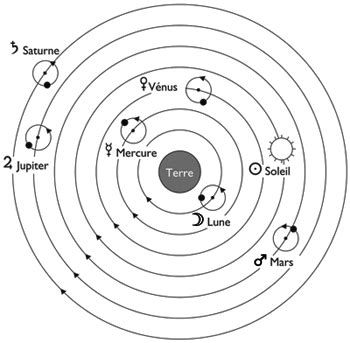
\includegraphics[scale=0.3]{./presentation/ptoleme}
\end{center}

\begin{center}
%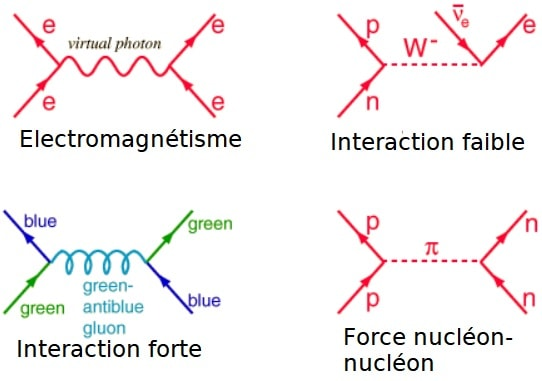
\includegraphics[scale=0.3]{./presentation/diagrammesInteractions}
\end{center}


% Author and supervisor
\begin{minipage}{0.4\textwidth}
\begin{flushleft} \large
%\emph{Auteur:}\\
%Stephan \textsc{Runigo}
\end{flushleft}
\end{minipage}
\begin{minipage}{0.4\textwidth}
\begin{flushright} \large
\emph{Auteur:}\\
Stephan \textsc{Runigo}
\end{flushright}
\end{minipage}

\vfill

% Bottom of the page
{\large \today}

\end{titlepage}

\newpage
\begin{center}
\Large
Résumé
\normalsize
\end{center}
\vspace{3cm}
\begin{itemize}[leftmargin=1cm, label=\ding{32}, itemsep=21pt]
\item {\bf Objet : } Souvenir des questions posés.
\item {\bf Contenu : } Définition, analyse, reflexion.
\item {\bf Public concerné : } Interressé à la question de l'âme.
\end{itemize}

\vspace{3cm}



\vspace{3cm}


%

%
% Table des matières
\tableofcontents
\thispagestyle{empty}
\setcounter{page}{0}
%
%espacement entre les lignes des tableaux
\renewcommand{\arraystretch}{1.5}
%
%====================== INCLUSION DES CHAPITRES ======================
%
~
\thispagestyle{empty}
%recommencer la numérotation des pages à "1"
\setcounter{page}{0}
\newpage
%
\chapter{Forces à distance}
%
Une force modélise une action mécanique : un homme pousse un chariot, le chariot se met en mouvement. L'action est de pousser, c'est une action de contact, son effet est la mise en mouvement. Cette action peut être modélisée par une force : l'homme applique une force sur le chariot.

\begin{center}

\includegraphics[scale=0.6]{./forces/chariotPousse}
\end{center}

Une force est représentée par un vecteur et un point d'application : Le point d'application est le point de contact (A), la force est horizontal, vers la droite et possède une valeur (mesurée en newton).

\begin{center}
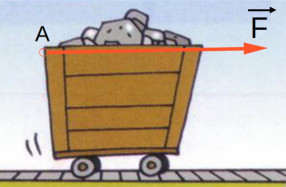
\includegraphics[scale=0.6]{./forces/chariotVecteur}
\end{center}

Nous étudions dans les paragraphes suivants, trois forces à distance (il n'y a pas de contact entre les corps).


%%%%%%%%%%%%%%%%%%%%%
\section{Force gravitationnelle}
%%%%%%%%%%%%%%%%%%%%%
%

L'interaction gravitationnelle est une action à distance entre les corps : les corps ayant une masse s'attirent entre eux, la force gravitationnelle modélise l'interaction gravitationnelle. 

La terre exerce sur la lune une action mécanique dont l'effet est d'{\it incurver} sa trajectoire, sans cette action la lune s'éloignerait de la terre.

\setlength{\unitlength}{1cm}
%
\begin{center}
\mbox{%\fbox{
\begin{picture}(17,3)
\put(2,2){\circle{1.52}}
\put(1.6,0.8){Terre}
\thicklines
\put(2,2){\vector(1,0){2.76}}
\put(4.3,2.3){$\overrightarrow{F}_{L/T}$}
\put(15,2){\circle{0.5}}
\put(14.6,1.2){Lune}
\thicklines
\put(15,2){\vector(-1,0){2.76}}
\put(12,2.3){$\overrightarrow{F}_{T/L}$}
\end{picture}}

$\overrightarrow{F_{L/T}}$ : Force gravitationnelle exercée par la lune sur la terre,

 $\overrightarrow{F_{T/L}}$ : Force gravitationnelle exercée par la terre sur la lune.
\end{center}


%%%%%%%%%%%%%%%%%%%%%%%%%%%%%%%%%%%%%%%%%%%%%%%%%%%%%%%%%%%%%%%%%%%%%%%%%%%%

%

%%%%%%%%%%%%%%%%%%%%%
\section{Champ électrique et potentiel scalaire}
%%%%%%%%%%%%%%%%%%%%%
%
Le champ électrique créé par une particule chargé s'étend dans l'espace à 3 dimensions. Il est possible, afin de simplifier les schéma de se limiter à 2 dimensions.

Le champ électrique créé par une particule chargée est radial et son amplitude décroit avec la distance à la particule.

\begin{center}
\tikzstyle{fleche}=[->,line width=1pt]
\begin{tikzpicture}
  \begin{scope}[xshift=0 cm,yshift=0 cm, scale = 1.6]%
\foreach \t in {60,120, ...,360}
\draw [fleche] (\t:1) -- (\t:2.8);
\foreach \t in {30,90, ...,360}
\draw [fleche] (\t:2) -- (\t:2.45);
\foreach \t in {15,45,-15,-45}
\draw [fleche] (\t:3) -- (\t:3.2);
\foreach \t in {15,45,-15,-45}
\draw [fleche] (\t+180:3) -- (\t+180:3.2);
\draw [fill=red] (0,0) circle(0.1) node [above right] {$Q_1$};
  \end{scope}
\end{tikzpicture}
\end{center}


Comme le champ de pente dérive d'un champ scalaire (le champ d'altitude), le champs electrique dérive d'un champ scalaire. On l'appelle le potentiel électrique. On représente ci-dessous les lignes de même potentiel (équi-potentiel) du potentiel électrique créé par une particule chargée.

\begin{center}
\begin{tikzpicture}
  \begin{scope}[xshift=0 cm,yshift=0 cm, scale = 1]%
\foreach \t in {1,2, ...,30}
\draw [line width=1pt] (0,0) circle (5/\t) ;

\draw [fill=red] (0,0) circle(0.2) node [above right,text=white] {$Q_1$};
  \end{scope}
\end{tikzpicture}
\end{center}

En 3 dimensions, les points de même potentiel sont des surfaces. Les surfaces équi-potentiel du potentiel créé par une particule chargée sont des sphères.

%%%%%%%%%%%%%%%%%%%%%%%%%%%%%%%%%%%%%%%%%%%%%%%%%%%%%%%%%%%%%%%%%%%%%%%%%%%%

%

%%%%%%%%%%%%%%%%%%%%%
\section{Force magnétique}
%%%%%%%%%%%%%%%%%%%%%
%

La force magnétique est la force qui s'exerce entre les \textbf{\textit {aimants}}.
Les aimants sont des matériaux possédant des propriétés magnétiques.
Certain métaux peuvent être aimantés par la proximité d'un aimant.

\subsection{Pôles magnétiques}

Un aimants est toujours {\it orienté}, il possède un pôle dit \textbf{\textit {nord}} et un pôle
dit \textbf{\textit {sud}}.


\subsection{Action magnétique}

La force magnétique entre deux aimants, est attractive et répulsive, elle exerce un {\it couple} :
entre deux aimants, les pôles opposés s'attirent, les pôles identiques se repoussent. 

Ci-dessous, deux aimants sont schématisés, les pôles nord en rouge et les pôles sud en bleu. On ne représente que les forces que l'aimant 2 exerce sur l'aimant 1.

\begin{center}
\begin{tikzpicture}[scale=1]
\fill [blue] (0,0) rectangle (0.3,1.5);
\fill [red] (0,1.5) rectangle (0.3,3);
\begin{scope}[rotate=30,yshift=-4.2cm]%
\fill [red] (8,0) rectangle (8.3,1.5);
\fill [blue] (8,1.5) rectangle (8.3,3);
\end{scope}
\thicklines
\put(0.15,0.15){\vector(1,0){1.76}}
\put(2,0.3){$\overrightarrow{F}_{N_2/S_1}$}

\put(0.15,2.85){\vector(1,0){2.26}}
\put(2.6,3){$\overrightarrow{F}_{S_2/N_1}$}

\draw [thick] [->] ((0.15,(0.15) --++(-1.5,-0.7) node [left] {$\overrightarrow{F}_{N_2/N_1}$};

\draw [thick] [->] ((0.15,(2.85) --++(-0.8,0.3) node [left] {$\overrightarrow{F}_{S_2/S_1}$};

%\put(0.15,0.15){\vector(-1,-1){0.5}}
%\put(4.3,2.3){$\overrightarrow{F}_{L/T}$}
\end{tikzpicture}
\end{center}
%%%%%%%%%%%%%%%%%%%%%%%%%%%%%%%%%%%%%%%%%%%%%%%%%%%%%%%%%%%%%%%%%%%%%%%%%%%%

%
%\input{.//.tex}

%

%%%%%%%%%%%%%%%%%%%%%
\section{Champs quantiques}
%%%%%%%%%%%%%%%%%%%%%
%
Une particule élémentaire est décrite par une fonction d'onde. Un ensemble de particules élémentaires identiques sont décrites par la superposition, la somme, des fonctions d'ondes individuelles. Ce champ total, pour un type de particule est à même de décrire l'ensemble de ces particules.

Ainsi, l'ensemble des électrons est décrit par le champ électron, l'ensemble des photons est décrit par le champ photon. Ces deux champs sont présent dans l'espace temps, la détection d'un photon ou d'un électron est due à un échange élémentaire d'énergie entre ces deux champs.

Lorsqu'un photon se matérialise en une paire électron-positron : un transfert d'énergie s'oppère du champ photon vers le champ électron. Lorsqu'un électron rencontre un positron, ils s'anihilent donnant un photon :  un transfert d'énergie s'oppère du champ électron vers le champ photon.

Une particule élémentaire peut alors être considérée comme l'évènement : transfert d'énergie entre deux champs quantique, la matière classique ne serait donc que la manifestation de ces évenements.

Les évènement de transfert d'énergie entre deux champs quantique caractérise le \textsf{\textit {couplage}} entre les champs.

L'existence (ou la détection) de la force électrique entre un électron et un proton serait la signature du couplage entre le champ électron et le champ photon d'une part et du couplage entre le champ proton et le champ photon. Le champ photon est le médiateur de la force électrique entre les particules chargées.
%%%%%%%%%%%%%%%%%%%%%%%%%%%%%%%%%%%%%%%%%%%%%%%%%%%%%%%%%%%%%%%%%%%%%%%%

%
\chapter{Champs et potentiel}
%
%

%%%%%%%%%%%%%%%%%%%%%
\section{Pente et altitude}
%%%%%%%%%%%%%%%%%%%%%
%
Le paysage ci-dessous est constitué de deux collines. La colline de gauche possède un coté très pentu. La colline de droite est moins haute. Un village se trouve à proximité du col.

\vfill
\begin{center}
\includegraphics[scale=0.7]{./potentiel/collines}
\end{center}

\vfill
Comment représenter ce paysage, qui est un relief en 3 dimensions, sur une carte en 2 dimensions ?

Nous allons voir deux façons de représenter ce relief : 

\vfill
\begin{minipage}[c]{.45\linewidth}
{\bf Les lignes de niveau} : c'est un champ scalaire (que l'on apellera champ d'altitude), donnant l'altitude du point considéré.

{\bf Les vecteurs "pente"} : c'est un champ vectoriel (que l'on apellera champ de pente), donnant la direction et l'importance de la pente (les vecteurs rouges ci-contre en donnent quelques exemples).
\end{minipage}
\hfill
\begin{minipage}[c]{.45\linewidth}
\begin{center}
\includegraphics[scale=0.4]{./potentiel/altitude}
\end{center}
\end{minipage}

\vfill
\newpage
%Sur une carte topographique, les lignes de niveaux sont utilisées. Alors que la surface de la terre est en 3 dimensions, 
%Une carte routière en 2 dimensions montre une vue de dessus suffisante. Sur une carte topographique, l'altitude est représenté en plus de la vue de dessus grâce aux lignes de niveau.

\subsection{"Champ d'altitude"}

Sur une carte topographique, le relief est représenté par des lignes de niveau, des lignes de même altitude.

Sur le schéma suivant, le paysage précédent est représenté vu de dessus. Son relief y est représenté à l'aide des lignes de niveau.

Les points d'altitudes 300 m, 350 m , et 400 m se trouve sur les lignes en gras en gras, les lignes en trait fin indiquent les points d'altitudes intermédiaires multiple de 10 (310 m, 320 m, 330 m, etc...)

%\vfill
\begin{center}
\includegraphics[scale=0.6]{./potentiel/potentiel}
\end{center}

%\vfill

En chaque point de la carte, on peut lire l'altitude en s'aidant des lignes de niveau (Le village se trouve à une altitude d'environ 295 m). Les lignes de niveau représentent donc un champ (le "champ d'altitude") dans un espace a 2 dimension (la carte), il s'agit d'un champ scalaire (l'altitude est un nombre).

Ces lignes sont plus proches les unes des autres lorsque la pente est plus forte.

%Nous allons voir qu'il existe une autre représentation du relief : le "champs de pente".

\vfill
\newpage
\subsection{"Champ de pente"}

Le "champs de pente" est un champ vectoriel, en chaque point de la carte, on représente la pente par un vecteur dirigé dans le sens de la pente et dont la longueur est proportionnel à la pente (d'autant plus grande que la pente est grande).

Le schéma ci-dessous représente le "vecteur pente" en quelques points de la carte. On constate que celui-ci est "grand" dans la zone pentu de la colline de gauche.

%\vfill
\begin{center}
\includegraphics[scale=0.7]{./potentiel/vecteur}
\end{center}

%\vfill
On remarque alors que le vecteur "champs de pente" est perpendiculaire au ligne de niveau du champs "d'altitude".

\vfill
\newpage
%%%%%%%%%%%%%%%%%%%%%%%%%%%%%%%%%%%%%%%%%%%%%%%%%%%%%%%%%%%%%%%%%%%%%%%%%%%%

%

%%%%%%%%%%%%%%%%%%%%%
\section{Champ électrique et potentiel scalaire}
%%%%%%%%%%%%%%%%%%%%%
%
Le champ électrique créé par une particule chargé s'étend dans l'espace à 3 dimensions. Il est possible, afin de simplifier les schéma de se limiter à 2 dimensions.

Le champ électrique créé par une particule chargée est radial et son amplitude décroit avec la distance à la particule.

\begin{center}
\tikzstyle{fleche}=[->,line width=1pt]
\begin{tikzpicture}
  \begin{scope}[xshift=0 cm,yshift=0 cm, scale = 1.6]%
\foreach \t in {60,120, ...,360}
\draw [fleche] (\t:1) -- (\t:2.8);
\foreach \t in {30,90, ...,360}
\draw [fleche] (\t:2) -- (\t:2.45);
\foreach \t in {15,45,-15,-45}
\draw [fleche] (\t:3) -- (\t:3.2);
\foreach \t in {15,45,-15,-45}
\draw [fleche] (\t+180:3) -- (\t+180:3.2);
\draw [fill=red] (0,0) circle(0.1) node [above right] {$Q_1$};
  \end{scope}
\end{tikzpicture}
\end{center}


Comme le champ de pente dérive d'un champ scalaire (le champ d'altitude), le champs electrique dérive d'un champ scalaire. On l'appelle le potentiel électrique. On représente ci-dessous les lignes de même potentiel (équi-potentiel) du potentiel électrique créé par une particule chargée.

\begin{center}
\begin{tikzpicture}
  \begin{scope}[xshift=0 cm,yshift=0 cm, scale = 1]%
\foreach \t in {1,2, ...,30}
\draw [line width=1pt] (0,0) circle (5/\t) ;

\draw [fill=red] (0,0) circle(0.2) node [above right,text=white] {$Q_1$};
  \end{scope}
\end{tikzpicture}
\end{center}

En 3 dimensions, les points de même potentiel sont des surfaces. Les surfaces équi-potentiel du potentiel créé par une particule chargée sont des sphères.

%%%%%%%%%%%%%%%%%%%%%%%%%%%%%%%%%%%%%%%%%%%%%%%%%%%%%%%%%%%%%%%%%%%%%%%%%%%%

%

%%%%%%%%%%%%%%%%%%%%%
\section{Force magnétique}
%%%%%%%%%%%%%%%%%%%%%
%

La force magnétique est la force qui s'exerce entre les \textbf{\textit {aimants}}.
Les aimants sont des matériaux possédant des propriétés magnétiques.
Certain métaux peuvent être aimantés par la proximité d'un aimant.

\subsection{Pôles magnétiques}

Un aimants est toujours {\it orienté}, il possède un pôle dit \textbf{\textit {nord}} et un pôle
dit \textbf{\textit {sud}}.


\subsection{Action magnétique}

La force magnétique entre deux aimants, est attractive et répulsive, elle exerce un {\it couple} :
entre deux aimants, les pôles opposés s'attirent, les pôles identiques se repoussent. 

Ci-dessous, deux aimants sont schématisés, les pôles nord en rouge et les pôles sud en bleu. On ne représente que les forces que l'aimant 2 exerce sur l'aimant 1.

\begin{center}
\begin{tikzpicture}[scale=1]
\fill [blue] (0,0) rectangle (0.3,1.5);
\fill [red] (0,1.5) rectangle (0.3,3);
\begin{scope}[rotate=30,yshift=-4.2cm]%
\fill [red] (8,0) rectangle (8.3,1.5);
\fill [blue] (8,1.5) rectangle (8.3,3);
\end{scope}
\thicklines
\put(0.15,0.15){\vector(1,0){1.76}}
\put(2,0.3){$\overrightarrow{F}_{N_2/S_1}$}

\put(0.15,2.85){\vector(1,0){2.26}}
\put(2.6,3){$\overrightarrow{F}_{S_2/N_1}$}

\draw [thick] [->] ((0.15,(0.15) --++(-1.5,-0.7) node [left] {$\overrightarrow{F}_{N_2/N_1}$};

\draw [thick] [->] ((0.15,(2.85) --++(-0.8,0.3) node [left] {$\overrightarrow{F}_{S_2/S_1}$};

%\put(0.15,0.15){\vector(-1,-1){0.5}}
%\put(4.3,2.3){$\overrightarrow{F}_{L/T}$}
\end{tikzpicture}
\end{center}
%%%%%%%%%%%%%%%%%%%%%%%%%%%%%%%%%%%%%%%%%%%%%%%%%%%%%%%%%%%%%%%%%%%%%%%%%%%%

%
%\input{./potentiel/.tex}
%

%
\chapter{Unification}
%

%%%%%%%%%%%%%%%%%%%%%
\section{Unification électromagnétique}
%%%%%%%%%%%%%%%%%%%%%
%

Oersted : Un courant électrique crée un champ magnétique

? : Un aimant en mouvement crée un champ magnétique.

Équation de Maxwell : Un champ magnétique variable au cours du temps crée un champ électrique, un champ électrique variable au cours du temps crée un champ magnétique.




%%%%%%%%%%%%%%%%%%%%%%%%%%%%%%%%%%%%%%%%%%%%%%%%%%%%%%%%%%%%%%%%%%%%%%%%

%

%%%%%%%%%%%%%%%%%%%%%
\section{Champ électromagnétique et espace-temps}
%%%%%%%%%%%%%%%%%%%%%
%
Les équations de Maxwell ne sont pas compatibles avec la structure newtonienne de l'espace temps. L'hypothèse de ces équations implique une structure einsteinienne de l'espace temps.



%%%%%%%%%%%%%%%%%%%%%%%%%%%%%%%%%%%%%%%%%%%%%%%%%%%%%%%%%%%%%%%%%%%%%%%%

%
%\input{./unification/.tex}

%

%
\chapter{La physique quantique}
%

%%%%%%%%%%%%%%%%%%%%%%%%%%%%%%%%%%%%%%%%%%%%

\section{Définitions}
  \subsection{Observateur et référentiel}

Pour étudier un mouvement, un {\it observateur} doit mesurer la position de l'objet en mouvement au cours du temps. Il doit donc disposer d'une horloge (pour mesurer le temps) et d'un système de coordonnées spatiales (pour mesurer la position).

L'horloge et le système de coordonnées "attachés" à l'observateur est appelé {\it référentiel}


    \subsubsection{Exemple}
Un observateur détermine la vitesse du train en chronomètrant la durée mis par le train pour parcourir la distance séparant les deux arbres.

\begin{center}
%%%%%%%%%%%%%%%%%%%%%%%%%%%%%%%%%%%%%%%%%%%%%%%%%%%%%%%
%%%%%%%%%%%%%%%%%%%%%%%%%%%%%%%%%%%%%%%%%%%%%%%%%%%%%%%%%%%%%%%%%%%%
\def\scl{0.2}%scaling factor of the picture

\begin{tikzpicture}[
  scale=\scl,
  beige/.style={color=gray!20!brown!40!yellow!20!},
  orange/.style={color=red!70!yellow!70!},
  wagon/.style={green!70!brown!20!black!75!,draw=black,thick},
  porte/.style={red!70!yellow!70!,draw=gray!20!, ultra thin},
  porteMotrice/.style={rounded corners = .1pt,draw=gray!60!, ultra thin},
  essieux/.style={gray!20!brown!30!black!60!,draw=black!70!, ultra thin},
  vitre/.style={bottom color=gray!5!, top color=gray!90!, shading angle={90}, draw=white, ultra thin},
  grisEssieux/.style={gray!20!brown!30!black!60!}
]


  \shade[bottom color=blue!20!white, top color=cyan!60!black] (20,10)
    rectangle (-60,0);
  \shade[bottom color=green!60!black, top color=green!60!] (20,-5)
    rectangle (-60,.3);



  \begin{scope}[xshift=0 cm,yshift=0 cm]%, scale = 0.3
%
%         LIAISONS
%
 \draw[black!70!, very thin] % liaison souple 42, rigide 65 +-11
    (6.1,0.65) to[out=330,in=0] (6.3,0.53);

 \draw[black!70!, very thin] 
    (-6.1,0.65) to[out=210,in=0] (-6.55,0.53);

 \draw[black!70!, thin] 
    (-6.1,0.76) -- (-6.56,0.76);


 % BUTOIRS
 %(\t * 6.1, 0.75) rectangle (\t * 6.4, 0.9);
 %(\t * 6.4, 0.7) rectangle (\t * 6.45, 0.95);

 % ESSIEUX derrière les roues

  \foreach \x in {3.64, -3.64}
   {
 \fill[gray] 
  (\x - 0.65, 0.95) -- (\x + 0.65, 0.95) --
 (\x + 1.6, 0.27) -- (\x + 1.06, 0.15) -- (\x + 0.65, 0.25)
 -- (\x - 0.65, 0.25) -- (\x - 1.06, 0.15) -- (\x - 1.6, 0.27) -- cycle;
  }

%  ROUES

\def\hauteur{0.55}% de l'axe des roues
\foreach \x in {2.58, 4.7, -4.7, -2.58}
  {
 % gris essieux : gray!20!brown!30!black!50!
    \fill[gray!20!brown!20!black!60!] (\x, \hauteur) circle (0.45 cm);
    \fill[gray!20!brown!40!black!40!] (\x, \hauteur) circle (0.41 cm);
    \fill[gray!10!brown!30!black!60!] (\x, \hauteur) circle (0.38 cm);

% RESSORT

  \foreach \t in {-1,1}
  {
     \draw[decorate, decoration={snake, segment length=1.5pt, amplitude=1.2mm}, black!70!, thin]
       (\x + \t * 0.28, 0.75) -- (\x + \t * 0.28, 0.35);
    % RESSORT fixation supérieur
     \fill[gray!20!brown!20!black!70!]
       (\x + \t * 0.28 - .13, 0.9) rectangle (\x + \t * 0.28 + .13, 0.7);
  }
  }


 % ESSIEUX devant les roues

\def\y{0.2}
  \foreach \x in {3.64, -3.64}
{
  \foreach \t in {-1,1}
  {
  % détail
 \fill[essieux] (\x + \t*1.57, 0.95) -- (\x + \t*1.67, 0.45) --
 (\x + \t*1.57, 0.45) -- (\x + \t*1.4, 0.95) -- cycle;

  %  montants supérieur
 \fill[essieux] (\x + \t*1.5, 0.95) -- (\x + \t*1.5, 0.85) -- (\x + \t*1, 0.83) -- (\x + \t*0.67, 0.65)
 -- (\x + \t*0.6, 0.35) -- (\x + \t*0.45, 0.35) -- (\x + \t*0.6, 0.95) -- cycle;


    %  montant inférieur
 \fill[essieux] (\x + \t * 1.5,0.45) -- (\x + \t * 1.5,0.4) -- (\x + \t * 1.2,0.35) -- (\x + \t * 1,0.35)
 -- (\x + \t * 0.80,0.37) -- (\x + \t * 0.65,0.25) -- (\x + \t * 0.65,0.45) -- cycle;

 \fill[essieux] (\x + \t*1.06, \hauteur + 0.05) circle (0.17 cm);
 \fill[grisEssieux]
 (\x + \t*1.06 + 0.16, 0.45) rectangle (\x + \t*1.06 + -0.16, 0.37);
 \fill[essieux]
 (\x + \t*1.06 + 0.1, \hauteur + 0.05 + -0.1) rectangle (\x + \t*1.06 + -0.1, \hauteur + 0.05 + 0.1);
    \fill[essieux] (\x + \t*1.06, \hauteur + 0.05) circle (0.09 cm);
    \fill[essieux] (\x + \t*1.06, \hauteur + 0.05) circle (0.04 cm);

  }

    %  milieux
   \fill[essieux, rounded corners = 3pt]
  (\x-0.22, 0.9) -- (\x + 0.22, 0.9) -- (\x + 0.4, 0.4) -- (\x - 0.4, 0.4) -- cycle;

    %  milieux inférieur 
  \fill[grisEssieux]
  (\x - 0.62,0.5) -- (\x + 0.62,0.5) -- (\x + 0.62,0.25) -- (\x - 0.62,0.25) -- cycle;

  \foreach \t in {-1,1}    % silent bloc
  {
  \fill[brown!30!black!80!]
 (\x + \t * 0.42 - 0.1, 0.6) rectangle (\x + \t * 0.42 + 0.1, 0.4);
  \fill[essieux]
 (\x + \t * 0.42 - 0.1, 0.45) rectangle (\x + \t * 0.42 + 0.1, 0.3);
  }
}

 % DESSOUS

 \fill[black!60!] 
  (1.9, 0.95) -- (- 1.9, 0.95) -- (- 1.4, 0.40) -- (1.4, 0.40) -- cycle;

  \shade[bottom color=gray!10!brown!50!black!60!, top color=gray!20!brown!40!black!40!] % ombre centre cylindre
  (1.05, 0.45) rectangle (-1.05, 0.66);
  \shade[bottom color=gray!20!brown!40!black!40!, top color=gray!10!brown!30!black!60!]
  (1.05, 0.64) rectangle (-1.05, 0.85);

 \fill[black!60!] 
  (2, 0.9) -- (- 2, 0.9) -- (- 1.9, 0.75) -- (1.9, 0.75) -- cycle;
 \fill[black!60!] 
  (1.15, 0.55) -- (- 1.15, 0.55) -- (- 1.15, 0.3) -- (1.15, 0.3) -- cycle;


  \shade[bottom color=brown!40!black!80!, top color=gray!20!brown!40!black!40!, rounded corners = 3pt]% cylindre
  (1.05, 0.45) rectangle (-1.05, 0.66);
  \shade[bottom color=gray!20!brown!40!black!40!, top color=gray!10!brown!30!black!60!, rounded corners = 3pt]%, shading angle={90}
  (1.05, 0.64) rectangle (-1.05, 0.85);

  \foreach \t in {-1,1}
{
  \fill[essieux] % details 1
 (\t * 2, 0.9) -- (\t * 1.7, 0.9) -- (\t * 1.72, 0.5)
 -- (\t * 1.85, 0.5) --  cycle;
  \fill[essieux] % details 2
 (\t * 1.67, 0.9) -- (\t * 1.2, 0.9) -- (\t * 1.2, 0.45)
 -- (\t * 1.67, 0.45) --  cycle;
}

 % BUTOIRS
\foreach \t in {-1,1}
{
  \fill[color=gray!80!black] % 
 (\t * 6.1, 0.75) rectangle (\t * 6.4, 0.9);
  \fill[color=black!80!gray] % plaques
 (\t * 6.4, 0.7) rectangle (\t * 6.45, 0.95);
}

% BAS DE CAISSE

\foreach \t in {-1,1}
{

  \fill[essieux] % details
 (\t * 5.9, 0.9) -- (\t * 5.3, 0.9) -- (\t * 5.5, 0.3)
 -- (\t * 5.85, 0.3) --  cycle;

  \fill[essieux] % pare bufle
 (\t * 6.2, 0.43) -- (\t * 6.35, 0.33) -- (\t * 6.2, 0.3) --  cycle;
  \fill[grisEssieux] % pare bufle
 (\t * 5, 0.95) -- (\t * 6.2, 0.95) -- (\t * 6.2, 0.3) --  cycle;

  \fill[color=gray] % carrosserie
 (\t * 5, 0.95) -- (\t * 6.2, 0.95) -- (\t * 6.2, 0.6) --  cycle;
}


%
%     CORPS DE LA MOTRICE
%
% liaisons électriques entre caténaires
     \draw[black!70!, thin] (-2.4, 3.15) -- (3.9, 3.15);

     \draw[black!70!, thin] (-4.5, 3.05) -- (4.1, 3.05);


%isolant 1
  \foreach \x in {-4.1, -3.6, 3.6, 4.1}
     \draw[decorate, decoration={snake, segment length=.2pt, amplitude=0.2mm}, red!50!black, thin]
       (\x, 2.9) -- (\x, 3.15);
  \foreach \x in {-4.1, -3.6, 3.6, 4.1}
     \fill[gray]
       (\x - 0.1, 2.9) rectangle (\x + 0.1, 2.95);

%caténaire
\def\h{0.05}
  \foreach \x in {-4.1, 3.6}
  {
     \draw[gray, line width=.7pt] (\x + 0.6, 3.1+\h) -- (\x - 0.1, 3.1+\h);
     \draw[black!60!, line width=1pt] (\x + 0.5, 3.15+\h) -- (\x, 3.15+\h);

     \draw[gray, line width=.7pt] (\x + 0.55, 3.05+\h) -- (\x + 1.8, 3.1+\h);
     \draw[gray, line width=.1pt] (\x + 0.55, 3.13+\h) -- (\x  + 1.8, 3.13+\h);

     \draw[gray, line width=.3pt] (\x, 3.2+\h) -- (\x  + 1.8, 3.15+\h);
     \draw[gray, line width=.1pt] (\x, 3.2+\h) -- (\x  + .8, 3.25+\h) -- (\x  + 1.7, 3.2+\h);
     \draw[gray, line width=.3pt] (\x  + .8, 3.18+\h) -- (\x  + .8, 3.28+\h);

  \fill[gray, draw=black!70!, thin, rounded corners = 1pt]% coude
 (\x + 1.8, 3.05+\h) -- (\x + 1.83, 3.1+\h) -- (\x + 1.78, 3.2+\h) -- (\x + 1.65, 3.2+\h)
 -- (\x + 1.68, 3.15+\h) -- cycle;

  }
  \foreach \x in {-4, 3.7}
  {
  \fill[gray, line width=2pt]% support et capteurs
 (\x-0.1, 3.28+\h) -- (\x+0.1, 3.28+\h) -- (\x, 3.17+\h)  -- cycle;
     \draw[gray, line width=.7pt] (\x-0.07, 3.28+\h) -- (\x-0.13, 3.28+\h);
     \draw[gray, line width=.7pt] (\x+0.07, 3.28+\h) -- (\x+0.13, 3.28+\h);
  }

% ÉLÉMENTS CATÉNAIRES

%isolant 2 à gauche
  \foreach \x in {-2.1, -2.35}
     \draw[decorate, decoration={snake, segment length=.2pt, amplitude=.4mm}, red!50!black, thin]
       (\x, 2.9) -- (\x, 3.15);
     \fill[gray] (-2.23 - 0.3, 2.9) rectangle (-2.23 + 0.3, 2.95);
     \fill[gray] (-2.23 - 0.3, 2.9) rectangle (-2.23 + 0.3, 2.95);
%isolant 2 à droite
     \draw[decorate, decoration={snake, segment length=.2pt, amplitude=.4mm}, red!50!black, thin]
       (2.6, 2.9) -- (2.6, 3.08);
   %  \fill[gray] (2.6 - 0.3, 2.9) rectangle (2.6 + 0.3, 2.95);
% boitier
  \foreach \x in {-4.6, 2.8}
{
     \draw[decorate, decoration={snake, segment length=.2pt, amplitude=0.1mm}, red!50!black, thin]
       (\x+0.25, 3.05) -- (\x+0.6, 3.05);

     \fill[gray] (\x - 0.28, 3.12) -- (\x + 0.28, 3.12)
     -- (\x + 0.3, 3.07)
     -- (\x + 0.28, 2.95) -- (\x - 0.28, 2.95) -- (\x - 0.3, 3.07) -- cycle;

     \draw[gray, ultra thick] (\x + 0.18, 3.12) -- (\x + 0.18, 2.5);
     \draw[gray, ultra thick] (\x, 3.12) -- (\x, 2.5);
}


% trompes
\foreach \t in {-1, 1}
  {
  \fill[gray]%
 (\t * 5.35,2.92) -- (\t * 5.75, 3) -- (\t * 5.75, 2.85)  -- cycle;
  \draw[gray, thin] (\t * 5.45, 3) -- (\t * 5.45, 2.85);
  }


% TOIT

  \fill[color=black!50!] % toit 1
 (1.9, 2.9) -- (-1.9, 2.9) -- (-1.65, 3.3) -- (1.65, 3.3) -- cycle;
\def\demi{0.25}
\foreach \x in{ -1.2, -0.6, 0, 0.6, 1.2 }
  \fill[black!30!] % grilles
 (\x - \demi, 3.1) rectangle (\x + \demi, 2.9);

  \fill[color=gray] % toit 2
 (4.5, 2.9) -- (5.75, 2.85) -- (5.85, 2.7) -- (-5.85, 2.7) -- 
 (-5.75, 2.85) -- (-4.5, 2.9) -- cycle;

  \fill[beige,draw=gray!50!, ultra thin] % carosserie
 (5.85, 2.7) -- (5.9, 2.55) -- (5.8, 2.1) -- (6.25, 1.95) -- (6.32, 1.75)
 -- (6.2, 0.9) --  (-6.2, 0.9) -- (-6.32, 1.75) -- (-6.25, 1.95)
 -- (-5.8, 2.1) -- (-5.9, 2.55) -- (-5.85, 2.7) -- cycle;

  \fill[orange] % décoration
 (4.45, 2.55) -- (3.85, 1.8) -- (6.32, 1.75) -- (6.35, 1.6) -- (3.35, 1.6) -- (4.1, 2.4) 
 -- (-4.1, 2.4) -- (-3.35, 1.6) -- (-6.27, 1.6) -- (-6.32, 1.75) -- (-3.85, 1.8) -- (-4.45, 2.55) -- cycle;


  \fill[color=gray!50!] % grille
 (3.2,1.6) -- (3.2, 2.4) -- (-3.2,2.4) -- (-3.2, 1.6) --  cycle;

  %  FEUX

\foreach \t in {-1,1}
{
  \fill[color=gray!50!,draw=gray, ultra thin]
 (\t * 6.3,1.67) rectangle (\t * 6.37, 1.53);
  \fill[color=brown!20!red!50!yellow!70!,draw=gray, ultra thin]
 (\t * 6.2,1.7) -- (\t * 6.3, 1.7) -- (\t * 6.3, 1.4) -- (\t * 6.1, 1.4) -- cycle;
  \fill[color=gray]
 (\t * 6.23,1.4) rectangle (\t * 6.28, 1.2);
}


\foreach \t in {-1,1}
{
      % PARE BRISE ET GRIS AUTOUR

  \fill[color=gray] % gris
 (\t*4.5, 2.55) -- (\t*5.9, 2.55) -- (\t*5.8, 2.1) -- (\t*4.15, 2.1) --  cycle;
  \shade[bottom color=gray!5!, top color=gray!90!, shading angle={90}, draw=black] % vitre
 (\t*5.8, 2.54) -- (\t*5.87, 2.54) -- (\t*5.8, 2.12) -- (\t*5.6, 2.12) --  cycle;

  \fill[color=gray] % gris
 (\t*4.5, 2.55) -- (\t*5.85, 2.55) -- (\t*5.65, 2.1) -- (\t*4.15, 2.1) --  cycle;

      % PORTES

    \draw[porteMotrice]
 (\t*4.55, 1.3) rectangle (\t*5, 2.6);

    \draw[draw=gray!40!,very thin] % marches
 (\t*4.62, 1.03) rectangle (\t*4.93, 1.15);

    \draw[color=gray] (\t*4.5, 1.03) -- (\t*4.5, 2.3); % rampes
    \draw[color=gray] (\t*5.05, 1.03) -- (\t*5.05, 2.3);

  \shade[bottom color=white, top color=black!80!, shading angle={90}]
   (\t*4.65, 2.12) rectangle (\t*4.9, 2.52); % vitres
}

  % RAIL

  % RAIL
  \fill[color=brown!20!gray!40!black]
 %(-8.75, 0.02) rectangle (8.75, -0.05); WAGON
 (20, 0.13) rectangle (-6.7, 0.06);

  \end{scope}
%
%
%%%%%%%%%%%%%%%%%%%%%%%%%%%%%%%%%%%%%%%%%%%%%%%%%%%%%%%%%%%%%%%%%%%%%

         %    WAGONS

%%%%%%%%%%%%%%%%%%%%%%%%%%%%%%%%%%%%%%%%%%%%%%%%%%%%%%%%%%%%%%%%%%%%

  \begin{scope}[xshift=-15.5 cm,yshift=0.11 cm]%, scale = 0.3
%
%         LIAISONS
% 
  \fill[color=gray,draw=gray!20!, ultra thin] % fixation souflets
 (8.65, 0.9) rectangle (-8.65, 2.2);

 \draw[black!70!, very thin] % liaison souple
    (8.3,0.65) to[out=330,in=180] (9,0.42);
 \draw[black!70!, very thin] 
    (-8.3,0.65) to[out=210,in=0] (-9,0.42);

  \foreach \t in {-1, 1}
  {
  \fill[color=black!80!,draw=gray!80!, ultra thin] % 
 (8.65 * \t, 0.9) rectangle (8.75 * \t, 2.3); % gris foncé, souflets

    \coordinate (A) at (8.3 * \t,0.65) ;
    \coordinate (B) at (9 * \t,0.65) ;
 \draw[black!70!, thin] 
    (A) -- (B);

  }

 % BUTOIRS
  \foreach \t in {-1, 1}
  {
  \fill[color=gray,draw=gray!50!, ultra thin] % 
 (8.3 * \t, 0.65) rectangle (\t * 8.66, 0.8);
  \fill[color=gray!50!black] % 
 (\t * 8.66, 0.6) rectangle (\t * 8.7, 0.85);
  }
%
%     CORPS DU WAGON
%
  \shade[bottom color=black!70!, top color=gray!50!, rounded corners=1pt]  % toit
 (-8.6, 2) rectangle (8.6, 2.7);

  \fill[color=gray!20!] % gris clair
 (-8.6, 2.1) rectangle (8.6, 2.4);
  \fill[color=gray!20!] % gris clair
 (-8.6, 0.8) rectangle (8.6, 1.25);

  \fill[color=gray!5!] % blanc
 (-8.6, 2.1) rectangle (8.6, 2.2);
  \fill[color=gray!5!] % blanc
 (-8.6, 1.25) rectangle (8.6, 1.3);

%  ROUES

\def\hauteur{0.35}% de l'axe des roues
\foreach \x in {5.45, 7.1, -5.45, -7.1}
  {
 % gris essieux : gray!20!brown!30!black!50!
    \fill[gray!20!brown!20!black!60!] (\x, \hauteur) circle (0.35 cm);
    \fill[gray!20!brown!40!black!40!] (\x, \hauteur) circle (0.31 cm);
    \fill[gray!10!brown!30!black!60!] (\x, \hauteur) circle (0.28 cm);
  \fill[color=gray,draw=black!70!, ultra thin] %,rotate=45
 (\x + 0.1, \hauteur + -0.1) rectangle (\x -0.1, \hauteur + 0.1);

  \fill[color=gray,draw=gray!20!, ultra thin] (\x, \hauteur) circle (0.08 cm);
  }
 % ESSIEUX
\def\y{0.2}
  \foreach \x in {6.25, -6.25}
   {
 \fill[black!20!gray!70!,draw=gray!20!, ultra thin] 
  (\x - 0.35, 0.2) rectangle (\x + 0.35, 0.45);

 \fill[black!20!gray!70!,draw=gray!20!, ultra thin] 
  (\x - 0.45, 0.45) rectangle (\x + 0.45, 0.55);

 \fill[black!20!gray!70!,draw=gray!20!, ultra thin] 
  (\x - 0.35, 0.55) rectangle (\x + 0.35, 0.7);

    \coordinate (A) at (\x + -0.75,\y + 0.45) ;
      \coordinate (B) at (\x - 0.2,\y + 0.27) ;
      \coordinate (C) at (\x + 0.2,\y + 0.27) ;
    \coordinate (D) at (\x + 0.75,\y + 0.45) ;
    \coordinate (E) at (\x + 0.75,\y + 0.32) ;
      \coordinate (F) at (\x + 0.2,\y + 0) ;
      \coordinate (G) at (\x - 0.2,\y + 0) ;
    \coordinate (H) at (\x - 0.75,\y + 0.32) ;
 \fill[black!20!gray!70!,draw=gray!20!, ultra thin] 
    (A) to[out=0,in=180] (B) to[out=0,in=180] (C) to[out=0,in=180]
    (D) to[out=-90,in=90] (E) to[out=180,in=0] (F) to[out=180,in=0]
    (G) to[out=180,in=0] (H) -- cycle;
  }

% MARCHE
  \foreach \t in {-1, 1}
  {
    \draw[draw=black!70!,very thin] % montant
 (\t * 7.9, 0.35) -- (\t * 7.8, 0.6);
    \draw[draw=black!70!,very thin] % montant
 (\t * 7.4, 0.35) -- (\t * 7.5, 0.6);
    \draw[draw=black!70!,thin] % marche
 (\t * 7.3, 0.35) -- (\t * 8, 0.35);
  }

% BAS DE CAISSE

  \fill[color=gray, rounded corners=1pt] % gris Foncé
    (-8.6, .8) rectangle (8.6, .65);


  \foreach \t in {-1, 1}
  \fill[color=gray, rounded corners=1pt] % gris Foncé
    (\t * 8.6, .7) -- (\t * 8.4, .45) -- (\t * 6.8, .45) -- (\t * 6.8, .7) -- cycle;
  \fill[color=gray, rounded corners=1pt] % gris Foncé
    (5.6, .7) -- (5.5, .45) -- (-5.5, .45) -- (-5.6, .7) -- cycle;

      % FENÊTRES
  \foreach \t in {1.05, 2.55, 4.05, 5.55}
  {
  \shade[vitre]
   (\t, 1.36) rectangle (\t + 1, 2.03);
  \shade[vitre]
   (-\t, 1.36) rectangle (-\t - 1, 2.03);
  }
  \shade[vitre]
   (-0.5, 1.36) rectangle (0.5, 2.03);

      % PORTES
  \foreach \t in {-1, 1}
  {

    \fill[gray!80!black] % marche
 (\t * 7.45, 0.53) rectangle (\t * 7.9, 0.7);
    \fill[gray!60!black] % marche
 (\t * 7.45, 0.53) rectangle (\t * 7.9, 0.57);

  \fill[gray!80!black]
 (\t * 7.2, 0.7) rectangle (\t * 8, 2.15);
  \fill[porte]
 (\t * 7.25, 0.8) rectangle (\t * 7.6, 2.05);
  \fill[porte]
 (\t * 7.45, 0.8) rectangle (\t * 7.9, 2.05);

  \shade[bottom color=gray!5!, top color=gray!90!, shading angle={90}, draw=black, ultra thin] % fenêtre
   (\t * 7.6, 1.4) rectangle (\t * 7.8, 1.9);

    \draw[gray!10!]
 (\t * 7.75, 1.15) -- (\t * 7.85, 1.1); % poignée
  }

  % RAIL WAGON
  \fill[color=brown!20!gray!40!black]
 (-8.85, 0.02) rectangle (8.85, -0.05);

  \end{scope}
%
%
%
%%%%%%%%%%%%%%%%%%%%%%%%%%%%%%%%%%%%%%%%%%%%%%%%%%%%%%%%%%%%%%%%%%%%%

         %    WAGON  2

%%%%%%%%%%%%%%%%%%%%%%%%%%%%%%%%%%%%%%%%%%%%%%%%%%%%%%%%%%%%%%%%%%%%

  \begin{scope}[xshift=-33.2 cm,yshift=0.11 cm]%, scale = 0.3
%
%         LIAISONS
% 
  \fill[color=gray,draw=gray!20!, ultra thin] % fixation souflets
 (8.65, 0.9) rectangle (-8.65, 2.2);

 \draw[black!70!, very thin] % liaison souple
    (8.3,0.65) to[out=330,in=180] (9,0.42);
 \draw[black!70!, very thin] 
    (-8.3,0.65) to[out=210,in=0] (-9,0.42);

  \foreach \t in {-1, 1}
  {
  \fill[color=black!80!,draw=gray!80!, ultra thin] % 
 (8.65 * \t, 0.9) rectangle (8.75 * \t, 2.3); % gris foncé, souflets
    \coordinate (A) at (8.3 * \t,0.65) ;
    \coordinate (B) at (9 * \t,0.65) ;
 \draw[black!70!, thin] 
    (A) -- (B);
  }

  \fill[color=black!80!] % 
 (8.75, 0.95) rectangle (8.95, 2.25); % gris foncé, souflet liaison
 % BUTOIRS
  \foreach \t in {-1, 1}
  {
  \fill[color=gray,draw=gray!50!, ultra thin] % 
 (8.3 * \t, 0.65) rectangle (\t * 8.66, 0.8);
  \fill[color=gray!50!black] % 
 (\t * 8.66, 0.6) rectangle (\t * 8.7, 0.85);
  }
%
%     CORPS DU WAGON
%
  \shade[bottom color=black!70!, top color=gray!50!, rounded corners=1pt]  % toit
 (-8.6, 2) rectangle (8.6, 2.7);

  \fill[color=gray!20!] % gris clair
 (-8.6, 2.1) rectangle (8.6, 2.4);
  \fill[color=gray!20!] % gris clair
 (-8.6, 0.8) rectangle (8.6, 1.25);

  \fill[color=gray!5!] % blanc
 (-8.6, 2.1) rectangle (8.6, 2.2);
  \fill[color=gray!5!] % blanc
 (-8.6, 1.25) rectangle (8.6, 1.3);

%  ROUES

\def\hauteur{0.35}% de l'axe des roues
\foreach \x in {5.45, 7.1, -5.45, -7.1}
  {
 % gris essieux : gray!20!brown!30!black!50!
    \fill[gray!20!brown!20!black!60!] (\x, \hauteur) circle (0.35 cm);
    \fill[gray!20!brown!40!black!40!] (\x, \hauteur) circle (0.31 cm);
    \fill[gray!10!brown!30!black!60!] (\x, \hauteur) circle (0.28 cm);
  \fill[color=gray,draw=black!70!, ultra thin] %,rotate=45
 (\x + 0.1, \hauteur + -0.1) rectangle (\x -0.1, \hauteur + 0.1);

  \fill[color=gray,draw=gray!20!, ultra thin] (\x, \hauteur) circle (0.08 cm);
  }
 % ESSIEUX
\def\y{0.2}
  \foreach \x in {6.25, -6.25}
   {
 \fill[black!20!gray!70!,draw=gray!20!, ultra thin] 
  (\x - 0.35, 0.2) rectangle (\x + 0.35, 0.45);

 \fill[black!20!gray!70!,draw=gray!20!, ultra thin] 
  (\x - 0.45, 0.45) rectangle (\x + 0.45, 0.55);

 \fill[black!20!gray!70!,draw=gray!20!, ultra thin] 
  (\x - 0.35, 0.55) rectangle (\x + 0.35, 0.7);

    \coordinate (A) at (\x + -0.75,\y + 0.45) ;
      \coordinate (B) at (\x - 0.2,\y + 0.27) ;
      \coordinate (C) at (\x + 0.2,\y + 0.27) ;
    \coordinate (D) at (\x + 0.75,\y + 0.45) ;
    \coordinate (E) at (\x + 0.75,\y + 0.32) ;
      \coordinate (F) at (\x + 0.2,\y + 0) ;
      \coordinate (G) at (\x - 0.2,\y + 0) ;
    \coordinate (H) at (\x - 0.75,\y + 0.32) ;
 \fill[black!20!gray!70!,draw=gray!20!, ultra thin] 
    (A) to[out=0,in=180] (B) to[out=0,in=180] (C) to[out=0,in=180]
    (D) to[out=-90,in=90] (E) to[out=180,in=0] (F) to[out=180,in=0]
    (G) to[out=180,in=0] (H) -- cycle;
  }

% MARCHE
  \foreach \t in {-1, 1}
  {
    \draw[draw=black!70!,very thin] % montant
 (\t * 7.9, 0.35) -- (\t * 7.8, 0.6);
    \draw[draw=black!70!,very thin] % montant
 (\t * 7.4, 0.35) -- (\t * 7.5, 0.6);
    \draw[draw=black!70!,thin] % marche
 (\t * 7.3, 0.35) -- (\t * 8, 0.35);
  }

% BAS DE CAISSE

  \fill[color=gray, rounded corners=1pt] % gris Foncé
    (-8.6, .8) rectangle (8.6, .65);


  \foreach \t in {-1, 1}
  \fill[color=gray, rounded corners=1pt] % gris Foncé
    (\t * 8.6, .7) -- (\t * 8.4, .45) -- (\t * 6.8, .45) -- (\t * 6.8, .7) -- cycle;
  \fill[color=gray, rounded corners=1pt] % gris Foncé
    (5.6, .7) -- (5.5, .45) -- (-5.5, .45) -- (-5.6, .7) -- cycle;

      % FENÊTRES
  \foreach \t in {1.05, 2.55, 4.05, 5.55}
  {
  \shade[vitre]
   (\t, 1.36) rectangle (\t + 1, 2.03);
  \shade[vitre]
   (-\t, 1.36) rectangle (-\t - 1, 2.03);
  }
  \shade[vitre]
   (-0.5, 1.36) rectangle (0.5, 2.03);

      % PORTES
  \foreach \t in {-1, 1}
  {

    \fill[gray!80!black] % marche
 (\t * 7.45, 0.53) rectangle (\t * 7.9, 0.7);
    \fill[gray!60!black] % marche
 (\t * 7.45, 0.53) rectangle (\t * 7.9, 0.57);

  \fill[gray!80!black]
 (\t * 7.2, 0.7) rectangle (\t * 8, 2.15);
  \fill[porte]
 (\t * 7.25, 0.8) rectangle (\t * 7.6, 2.05);
  \fill[porte]
 (\t * 7.45, 0.8) rectangle (\t * 7.9, 2.05);

  \shade[bottom color=gray!5!, top color=gray!90!, shading angle={90}, draw=black, ultra thin] % fenêtre
   (\t * 7.6, 1.4) rectangle (\t * 7.8, 1.9);

    \draw[gray!10!]
 (\t * 7.75, 1.15) -- (\t * 7.85, 1.1); % poignée
  }

  % RAIL WAGON
  \fill[color=brown!20!gray!40!black]
 (-8.85, 0.02) rectangle (8.85, -0.05);

  \end{scope}
%
%
%%%%%%%%%%%%%%%%%%%%%%%%%%%%%%%%%%%%%%%%%%%%%%%%%%%%%%%%%%%%%%%%%%%%%

         %    WAGON  3

%%%%%%%%%%%%%%%%%%%%%%%%%%%%%%%%%%%%%%%%%%%%%%%%%%%%%%%%%%%%%%%%%%%%

  \begin{scope}[xshift=-50.9 cm,yshift=0.11 cm]%, scale = 0.3
%
%         LIAISONS
% 
  \fill[color=gray,draw=gray!20!, ultra thin] % fixation souflets
 (8.65, 0.9) rectangle (-8.65, 2.2);

 \draw[black!70!, very thin] % liaison souple
    (8.3,0.65) to[out=330,in=180] (9,0.42);

 \draw[black!70!, very thin] 
    (-8.3,0.65) -- (-8.6,0.45);

  \foreach \t in {-1, 1}
  {
  \fill[color=black!80!,draw=gray!80!, ultra thin] % 
 (8.65 * \t, 0.9) rectangle (8.75 * \t, 2.3); % gris foncé, souflets
  }
  \fill[color=black!80!] % 
 (8.75, 0.95) rectangle (8.95, 2.25); % gris foncé, souflet liaison

    \coordinate (A) at (8.3,0.65) ;
    \coordinate (B) at (9,0.65) ;
 \draw[black!70!, thin] 
    (A) -- (B);

 % BUTOIRS
  \foreach \t in {-1, 1}
  {
  \fill[color=gray,draw=gray!50!, ultra thin] % 
 (8.3 * \t, 0.65) rectangle (\t * 8.66, 0.8);
  \fill[color=gray!50!black] % 
 (\t * 8.66, 0.6) rectangle (\t * 8.7, 0.85);
  }
%
%     CORPS DU WAGON
%
  \shade[bottom color=black!70!, top color=gray!50!, rounded corners=1pt]  % toit
 (-8.6, 2) rectangle (8.6, 2.7);

  \fill[color=gray!20!] % gris clair
 (-8.6, 2.1) rectangle (8.6, 2.4);
  \fill[color=gray!20!] % gris clair
 (-8.6, 0.8) rectangle (8.6, 1.25);

  \fill[color=gray!5!] % blanc
 (-8.6, 2.1) rectangle (8.6, 2.2);
  \fill[color=gray!5!] % blanc
 (-8.6, 1.25) rectangle (8.6, 1.3);

%  ROUES

\def\hauteur{0.35}% de l'axe des roues
\foreach \x in {5.45, 7.1, -5.45, -7.1}
  {
 % gris essieux : gray!20!brown!30!black!50!
    \fill[gray!20!brown!20!black!60!] (\x, \hauteur) circle (0.35 cm);
    \fill[gray!20!brown!40!black!40!] (\x, \hauteur) circle (0.31 cm);
    \fill[gray!10!brown!30!black!60!] (\x, \hauteur) circle (0.28 cm);
  \fill[color=gray,draw=black!70!, ultra thin] %,rotate=45
 (\x + 0.1, \hauteur + -0.1) rectangle (\x -0.1, \hauteur + 0.1);

  \fill[color=gray,draw=gray!20!, ultra thin] (\x, \hauteur) circle (0.08 cm);
  }
 % ESSIEUX
\def\y{0.2}
  \foreach \x in {6.25, -6.25}
   {
 \fill[black!20!gray!70!,draw=gray!20!, ultra thin] 
  (\x - 0.35, 0.2) rectangle (\x + 0.35, 0.45);

 \fill[black!20!gray!70!,draw=gray!20!, ultra thin] 
  (\x - 0.45, 0.45) rectangle (\x + 0.45, 0.55);

 \fill[black!20!gray!70!,draw=gray!20!, ultra thin] 
  (\x - 0.35, 0.55) rectangle (\x + 0.35, 0.7);

    \coordinate (A) at (\x + -0.75,\y + 0.45) ;
      \coordinate (B) at (\x - 0.2,\y + 0.27) ;
      \coordinate (C) at (\x + 0.2,\y + 0.27) ;
    \coordinate (D) at (\x + 0.75,\y + 0.45) ;
    \coordinate (E) at (\x + 0.75,\y + 0.32) ;
      \coordinate (F) at (\x + 0.2,\y + 0) ;
      \coordinate (G) at (\x - 0.2,\y + 0) ;
    \coordinate (H) at (\x - 0.75,\y + 0.32) ;
 \fill[black!20!gray!70!,draw=gray!20!, ultra thin] 
    (A) to[out=0,in=180] (B) to[out=0,in=180] (C) to[out=0,in=180]
    (D) to[out=-90,in=90] (E) to[out=180,in=0] (F) to[out=180,in=0]
    (G) to[out=180,in=0] (H) -- cycle;
  }

% MARCHE
  \foreach \t in {-1, 1}
  {
    \draw[draw=black!70!,very thin] % montant
 (\t * 7.9, 0.35) -- (\t * 7.8, 0.6);
    \draw[draw=black!70!,very thin] % montant
 (\t * 7.4, 0.35) -- (\t * 7.5, 0.6);
    \draw[draw=black!70!,thin] % marche
 (\t * 7.3, 0.35) -- (\t * 8, 0.35);
  }

% BAS DE CAISSE

  \fill[color=gray, rounded corners=1pt] % gris Foncé
    (-8.6, .8) rectangle (8.6, .65);


  \foreach \t in {-1, 1}
  \fill[color=gray, rounded corners=1pt] % gris Foncé
    (\t * 8.6, .7) -- (\t * 8.4, .45) -- (\t * 6.8, .45) -- (\t * 6.8, .7) -- cycle;
  \fill[color=gray, rounded corners=1pt] % gris Foncé
    (5.6, .7) -- (5.5, .45) -- (-5.5, .45) -- (-5.6, .7) -- cycle;

      % FENÊTRES
  \foreach \t in {1.05, 2.55, 4.05, 5.55}
  {
  \shade[vitre]
   (\t, 1.36) rectangle (\t + 1, 2.03);
  \shade[vitre]
   (-\t, 1.36) rectangle (-\t - 1, 2.03);
  }
  \shade[vitre]
   (-0.5, 1.36) rectangle (0.5, 2.03);

      % PORTES
  \foreach \t in {-1, 1}
  {

    \fill[gray!80!black] % marche
 (\t * 7.45, 0.53) rectangle (\t * 7.9, 0.7);
    \fill[gray!60!black] % marche
 (\t * 7.45, 0.53) rectangle (\t * 7.9, 0.57);

  \fill[gray!80!black]
 (\t * 7.2, 0.7) rectangle (\t * 8, 2.15);
  \fill[porte]
 (\t * 7.25, 0.8) rectangle (\t * 7.6, 2.05);
  \fill[porte]
 (\t * 7.45, 0.8) rectangle (\t * 7.9, 2.05);

  \shade[bottom color=gray!5!, top color=gray!90!, shading angle={90}, draw=black, ultra thin] % fenêtre
   (\t * 7.6, 1.4) rectangle (\t * 7.8, 1.9);

    \draw[gray!10!]
 (\t * 7.75, 1.15) -- (\t * 7.85, 1.1); % poignée
  }

  % RAIL WAGON
  \fill[color=brown!20!gray!40!black]
 (-9.1, 0.02) rectangle (8.85, -0.05);

  \end{scope}
%
\tikzset{
  treetop/.style = {decoration={random steps, segment length=0.2mm}, decorate},
  trunk/.style   = {decoration={random steps, segment length=1mm,
                    amplitude=0.2mm}, decorate}}

%  arbre à droite
       \fill [brown!50!black, trunk] (15,-1) rectangle (15.8,2);
       \fill [brown!60!black, trunk] (15.2,-1) rectangle (15.6,2);
     
       \fill [green!60!black, treetop](15,3) ellipse (1.5 and 2.25);
       \fill [green!40!black, treetop](15,3) ellipse (1 and 1.5);
     

%  arbre à gauche
       \fill [brown!30!black, trunk] (-55,-1) rectangle (-55.8,3);
       \fill [brown!60!black, trunk] (-55.2,-1) rectangle (-55.6,3);
     
       \fill [green!60!black, treetop](-55,3) ellipse (1.5 and 2.25);
       \fill [green!40!black, treetop](-55,3) ellipse (1 and 1.5);
     

%
\end{tikzpicture}
%

%%%%%%%%%%%%%%%%%%%%%%%%%%%%%%%%%%%%%%%%%%%%%%%%%%%%%%
%%%%%%%%%%%%%%%%%%%%%%%%%%%%%%%%%%%%%%%%%%%%%%%%%%%%%%%%%%%%%%%%%%%%
\def\scl{1}%scaling factor of the picture


\begin{tikzpicture}[
  scale=\scl,
  %wagon/.style={yellow!30!brown!20!,rounded corners,draw=black,thick},
  wagon/.style={green!70!brown!20!black!75!,draw=black,thick},
 % toit/.style={black!70!brown!20!,draw=gray,thick},
  %roue/.style={brown!20!black!70!,draw=black,thick},
  fenetre/.style={white,rounded corners = 2pt,draw=black, thick},
  porte/.style={color=red!70!yellow!70!,draw=gray!50!, ultra thin}
  ]

  \begin{scope}[xshift=0 cm,yshift=0 cm]%, scale = 0.3
%
%         LIAISONS
% 
  \fill[color=gray,draw=gray!20!, ultra thin] % souflet gris
 (8.65, 0.9) rectangle (-8.65, 2.2);

 \draw[black!70!, very thick] 
    (8.3,0.65) to[out=330,in=180] (8.75,0.42);
 \draw[black!70!, very thick] 
    (-8.3,0.65) to[out=210,in=0] (-8.75,0.42);

  \foreach \t in {-1, 1}
  {
  \fill[color=black!80!,draw=gray!80!, ultra thin, rounded corners=2pt] % 
 (8.65 * \t, 0.9) rectangle (8.75 * \t, 2.3); % gris foncé, souflet

    \coordinate (A) at (8.3 * \t,0.65) ;
    \coordinate (B) at (8.75 * \t,0.65) ;
 \draw[black!70!, ultra thick] 
    (A) -- (B);

  }

 % BUTOIRS
  \foreach \t in {-1, 1}
  {
  \fill[color=gray,draw=gray!50!, ultra thin] % 
 (8.3 * \t, 0.65) rectangle (\t * 8.66, 0.8);
  \fill[color=gray!50!black] % 
 (\t * 8.66, 0.6) rectangle (\t * 8.7, 0.85);
  }
%
%     CORPS DU WAGON
%
  \shade[bottom color=gray, top color=gray!10!, rounded corners]  % toit
 (-8.6, 2) rectangle (8.6, 2.7);

  \fill[color=gray!20!] % gris clair
 (-8.6, 2.1) rectangle (8.6, 2.4);
  \fill[color=gray!20!] % gris clair
 (-8.6, 0.8) rectangle (8.6, 1.25);

  \fill[color=gray!5!] % blanc
 (-8.6, 2.1) rectangle (8.6, 2.2);
  \fill[color=gray!5!] % blanc
 (-8.6, 1.25) rectangle (8.6, 1.3);


% Arriere roues
  %\foreach \x in {6.25, -6.25} \fill[brown!40!black] (\x - 0.85, 0.8) rectangle (\x + 0.85, 0.45);

%  ROUES
\def\hauteur{0.35}% de l'axe des roues
\tikzset{
  roue/.pic={
    \fill[black!20!gray!70!] (0, \hauteur) circle (0.35 cm);
    \fill[gray!20!] (0, \hauteur) circle (0.31 cm);
    \fill[black!20!gray!70!] (0, \hauteur) circle (0.28 cm);

  \fill[color=gray,draw=gray!20!, ultra thin] %,rotate=45
 (0.1, \hauteur + -0.1) rectangle (-0.1, \hauteur + 0.1);

  \fill[color=gray,draw=gray!20!, ultra thin] (0, \hauteur) circle (0.08 cm);

  }
}

  \pic at (5.45,0)    {roue};
  \pic at (7.1,0)    {roue};
  \pic at (-5.45,0)    {roue};
  \pic at (-7.1,0)    {roue};
 % ESSIEUX
\def\y{0.2}
  \foreach \x in {6.25, -6.25}
   {
 \fill[black!20!gray!70!,draw=gray!20!, ultra thin] 
  (\x - 0.35, 0.2) rectangle (\x + 0.35, 0.45);

 \fill[black!20!gray!70!,draw=gray!20!, ultra thin] 
  (\x - 0.45, 0.45) rectangle (\x + 0.45, 0.55);

 \fill[black!20!gray!70!,draw=gray!20!, ultra thin] 
  (\x - 0.35, 0.55) rectangle (\x + 0.35, 0.7);

    \coordinate (A) at (\x + -0.75,\y + 0.45) ;
      \coordinate (B) at (\x - 0.2,\y + 0.27) ;
      \coordinate (C) at (\x + 0.2,\y + 0.27) ;
    \coordinate (D) at (\x + 0.75,\y + 0.45) ;
    \coordinate (E) at (\x + 0.75,\y + 0.32) ;
      \coordinate (F) at (\x + 0.2,\y + 0) ;
      \coordinate (G) at (\x - 0.2,\y + 0) ;
    \coordinate (H) at (\x - 0.75,\y + 0.32) ;
 \fill[black!20!gray!70!,draw=gray!20!, ultra thin] 
    (A) to[out=0,in=180] (B) to[out=0,in=180] (C) to[out=0,in=180]
    (D) to[out=-90,in=90] (E) to[out=180,in=0] (F) to[out=180,in=0]
    (G) to[out=180,in=0] (H) -- cycle;
  }

% MARCHE
  \foreach \t in {-1, 1}
  {
    \draw[draw=black!70!,very thick] % montant
 (\t * 7.9, 0.35) -- (\t * 7.8, 0.6);
    \draw[draw=black!70!,very thick] % montant
 (\t * 7.4, 0.35) -- (\t * 7.5, 0.6);
    \draw[draw=black!70!,thick] % marche
 (\t * 7.3, 0.35) -- (\t * 8, 0.35);
  }

% BAS DE CAISSE

  \fill[color=gray, rounded corners=1pt] % gris Foncé
    (-8.6, .8) rectangle (8.6, .65);


  \foreach \t in {-1, 1}
  \fill[color=gray, rounded corners=1pt] % gris Foncé
    (\t * 8.6, .7) -- (\t * 8.4, .45) -- (\t * 6.8, .45) -- (\t * 6.8, .7) -- cycle;
  \fill[color=gray, rounded corners=1pt] % gris Foncé
    (5.6, .7) -- (5.5, .45) -- (-5.5, .45) -- (-5.6, .7) -- cycle;

      % FENÊTRES
  \foreach \t in {1.05, 2.55, 4.05, 5.55}
  {
  \shade[bottom color=gray!5!, top color=gray!90!, shading angle={90},rounded corners=2pt, draw=white]
   (\t, 1.36) rectangle (\t + 1, 2.03);
  \shade[bottom color=gray!5!, top color=gray!90!, shading angle={90},rounded corners=2pt, draw=white]
   (-\t, 1.36) rectangle (-\t - 1, 2.03);
  }
  \shade[bottom color=gray!5!, top color=gray!90!, shading angle={90},rounded corners=2pt, draw=white]
   (-0.5, 1.36) rectangle (0.5, 2.03);

      % PORTES
  \foreach \t in {-1, 1}
  {

    \fill[gray!80!black] % marche
 (\t * 7.45, 0.53) rectangle (\t * 7.9, 0.7);
    \fill[gray!60!black] % marche
 (\t * 7.45, 0.53) rectangle (\t * 7.9, 0.57);

  \fill[gray!80!black]
 (\t * 7.2, 0.7) rectangle (\t * 8, 2.15);
  \fill[porte]
 (\t * 7.25, 0.8) rectangle (\t * 7.6, 2.05);
  \fill[porte]
 (\t * 7.45, 0.8) rectangle (\t * 7.9, 2.05);

  \shade[bottom color=gray!5!, top color=gray!90!, shading angle={90},rounded corners=2pt, draw=black] % fenêtre
   (\t * 7.6, 1.4) rectangle (\t * 7.8, 1.9);

    \draw[gray!10!]
 (\t * 7.75, 1.15) -- (\t * 7.85, 1.1); % poignée
  }

  % RAIL
  \fill[color=brown!20!gray!40!black]
 (-8.75, 0.02) rectangle (8.75, -0.05);

  \end{scope}
%
%
\end{tikzpicture}
%

\end{center}

L'observateur est immobile par rapport à la Terre, le mouvement est étudié dans le {\it référentiel terrestre}.

Un voyageur est assis dans le train, il observe le paysage défiler. Il se trouve dans le {\it référentiel lié au train} et peut également chronométrer la durée pour parcourir la distance entre les deux arbres, et ainsi déterminer la "vitesse du paysage" dans son régérentiel.


  \subsection{Mouvement rectiligne uniforme}

Un mouvement {\it rectiligne} est un mouvement en ligne droite. Un mouvement {\it uniforme} est un mouvement dont la vitesse est constante.

%%%%%%%%%%%%%%%%%%%%%%%%%%%%%%%%%%%%%%%%%%%{\it }




%
%
%%%%%%%%%%%%%%%%%%%%%%%%%%%%%%%%%%%%%%%%%%%%

\section{Initiation au diagrammes de Feynman \cite{diagrammesFeynman}}

%%%%%%%%%%%%%%%%%%%%%%%%%%%%%%%%%%%%%%%%%%%

\label{JeanLucDeziel}

\subsection{Définition}

Un diagramme de Feynman est généralement un graphe en 2 dimensions où l'un des axe est attribué à l'espace, l'autre au temps, et dans lequel on représente les interactions entre les particules élémentaires. 
 %et dans lequel on représente les interactions entre les champs.

%Les champs échangent de l'énergie entre eux de manière quantique, à travers les phénomènes de création (ou émission) et d'anihilation (ou absorption) des quantons.

%On suppose que l'on dispose de dispositif expérimental permettant de détecter les particules.

Une vision corpusculaire (granulaire) des quantons permet de se familiariser avec ces diagrammes. Les diagrammes représentent alors les "trajectoires" des quantons.

L'électron et le photon sont des quantons. L'électron possède une masse ainsi qu'une charge électrique (il est l'un des principaux constituant de la matière avec le proton et le neutron). Le photon est la "particule de la lumière". Il n'a ni masse ni charge électrique et il se déplace à la vitesse de la lumière. Les interactions entre les électrons se produisent par échange de photon.


\subsection{Exemple et conventions}

Dans les diagrammes, un électron est représenté par un segment muni d'une flêche, un photon est représenté par un segment ondulé.

Dans les diagrammes suivants, les chiffres 1, 2, 3 et 4 ont été rajoutés pour des raisons pédagogiques, ils facilitent les explications chronologique des diagrammes.
\vspace{0.9cm}

\tikzset{
electron/.style={postaction={decorate}, decoration={markings,mark=at position .6 with {\arrow[#1]{latex}}}},
%positon/.style={postaction={decorate}, decoration={markings,mark=at position .5 with {\arrow[#1]{latex}}}},
photon/.style={decorate, decoration={snake, segment length=8pt, amplitude=1.8pt}}
}
\begin{minipage}[c]{.45\linewidth}
\begin{tikzpicture}
% désactive les caractères pour babel ? %\shorthandoff{:;!?};[scale=1.5]
\begin{scope}[scale=0.7]
%Création des axes xy
    \draw[-latex, very thick] (0,0) -- (5,0) node[below] {espace};
    \draw[-latex, very thick] (0,0) -- (0,5) node[left] {temps};
% Définition des noeuds
    \coordinate (e1) at (1,1);
    \coordinate (e2) at (4,2);
    \coordinate (e3) at (2,2.5);
   \coordinate (e4) at (1.3,4);
% dessin des particules
\draw [electron, very thick] (e1) -- (e3);
\draw [electron, very thick] (e3) -- (e4);
\draw [photon, very thick] (e3) -- (e2);
% Nommage
  \draw (e1) node [below] {1};
  \draw (e2) node [right] {2};
  \draw (e3) node [above right] {3};
  \draw (e4) node [above] {4};
\end{scope}
%above, below, right, left,
%above left, above right, below left, below right
%au-dessus, en-dessous, à droite, à gauche
%au-dessus à gauche, au-dessus à droite, en-dessous à gauche, en-dessous à droite
%
\end{tikzpicture}
\end{minipage}
\hfill
\begin{minipage}[c]{.45\linewidth}
\begin{center}
Explication chronologique :
\end{center}
Un électron se déplace de 1 à 3, un photon se déplace de 2 à 3. En 3, l'électron absorbe le photon. Muni de ce regain d'énergie, l'électron se précipite en 4.
\end{minipage}


\subsection{Interaction électromagnétique}

Les électrons sont des particules chargés électriquement'interaction entre deux électrons

%\vspace{1.1cm}
\begin{minipage}[c]{.45\linewidth}
\begin{center}
Explication chronologique :
\end{center}
Un électron se déplace de 1 à 3 tandis qu'un autre électron se déplace de 2 à 4.

\end{minipage}
\hfill
\begin{minipage}[c]{.45\linewidth}
\begin{tikzpicture}
% désactive les caractères pour babel ? %\shorthandoff{:;!?};
\begin{scope}[scale=0.7]
%Création des axes xy
   \draw[-latex, very thick] (0,0) -- (5,0) node[below] {espace};
   \draw[-latex, very thick] (0,0) -- (0,5) node[left] {temps};
% Définition des noeuds
   \coordinate (e1) at (2,1);
   \coordinate (e2) at (3.5,1);
   \coordinate (e3) at (1,4);
   \coordinate (e4) at (4,4);
% dessin des particules
\draw [electron, very thick] (e1) -- (e3);
\draw [electron, very thick] (e2) -- (e4);
% Nommage
  \draw (e1) node [left] {1};
  \draw (e2) node [right] {2};
  \draw (e3) node [left] {3};
  \draw (e4) node [right] {4};
\end{scope}
%above, below, right, left,
%above left, above right, below left, below right
%au-dessus, en-dessous, à droite, à gauche
%au-dessus à gauche, au-dessus à droite, en-dessous à gauche, en-dessous à droite
%
\end{tikzpicture}
\end{minipage}

%%%%%%%%%%%%%%%%%%%%%%%%%%%%%%%%%%%%%%%%%%%%%%%%%%%%%%%%%%%%%%%%%%%%%%%%%%%%%

%

%%%%%%%%%%%%%%%%%%%%%
\chapter{Paradigmes}
%%%%%%%%%%%%%%%%%%%%%

\section{Mécanique Newtoniennne}
%
La trajectoire d'un corps est décrite par ses coordonnées évoluant au cours du temps, obéissant au lois de la mécanique.
%
\section{Mécanique quantique}

L'évolution au cours du temps d'un quanton est décrite par sa fonction d'onde donnant l'amplitude de probabilité de mesurer ce quanton (de l'observer). La fonction d'onde evolue suivant l'équation de Schrödinger.

\section{Théorie quantique des champs}

Les différents champs échangent de l'énergie entre eux de manière quantique.

%%%%%%%%%%%%%%%%%%%%%%%%%%%%%%%%%%%%%%%%%%%%%%%%%%%%%%%%%%%%%%%%%%%%%%%%%%%%%%%%%%%%%

%
%
%%%%%%%%%%%%%%%%%%%%%%%%%%%%%%%%%%%%%%%%%%%%

\section{Théorie des champs}

%%%%%%%%%%%%%%%%%%%%%%%%%%%%%%%%%%%%%%%%%%%

%\subsection{}

Finallement, le diagramme représentant un échange élémentaire d'énergie entre le champ électron et le champ photon est le suivant :

\begin{center}
\includegraphics[scale=2.5]{./quantique/feynmannElementaire}
\end{center}

Un tel échange se représente comme un processus unique qui apparaît tantôt comme une création, tantôt comme une anihilation, tantôt comme une émission, tantôt comme une absorption, suivant comment on place les axes de temps et d'espace.

%Ainsi, il semblerait que ce processus élémentaire d'interaction entre les champs se produirait sans existence prélable de temps et d'espace, mais faisant apparaître un temps et un espace à nos sens.

\subsection{Champs et quantons}

Les quantons n'apparaissent alors plus comme des "particules de matière" mais comme la "signature" des champs échangeant de l'énergie.

L'électromagnétisme quantique décrit donc les champs photon, électron et positron, comme trois champs "couplés". Ce couplage signifie qu'ils échangent de l'énergie entre eux. Cet échange se produit de façon quantique (quantifié, discrète, "atomique").

La nature nous apparaitrait comme quantifié car nous considérons comme "objet", non pas les champs, mais leurs échanges, leur couplage. La nature serait constitué de champs, continus, leur interaction discontinu nous faisant apparaître une nature "atomique".  

\subsection{Espace-temps et causalité}

Le diagramme élémentaire nous montre une unification des interactions entre les champs, dans laquelle l'espace et le temps jouerait un rôle "secondaire". On aurait plutôt à faire à des "évènements espacé" (échange quantique entre les champs) qui vérifiraient un "principe causal". L'espace-temps serait alors notre perception de ce monde d'évènements "espacés et causaux". en effet :

Ce qui ressort de l'espace-temps des physiciens, c'est principalement l'invariance de la vitesse de la lumière, l'espace et le temps sont reliés, ce qui est fondamental semble être leur "liens", la vitesse limite.

La vitesse limite peut apparaître comme la "signature" d'un principe de causalité auquel obéirait les champs.
%%%%%%%%%%%%%%%%%%%%%%%%%%%%%%%%%%%%%%%%%%%%%%%%%%%%%%%%%%%%%%%%%%%%%%%%%%%%%

%
%\input{./quantique/feynmann.tex}
%
%

%
%
\begin{appendix}
%

%%%%%%%%%%%%%%%%%%%%%
\chapter{Glossaire}
%%%%%%%%%%%%%%%%%%%%%

\begin{itemize}[leftmargin=1cm, label=\ding{32}, itemsep=2pt]
\item {\bf application} : en mathématique, synonyme de fonction.
\item {\bf } :
\item {\bf } :
\item {\bf quanton} : particule élémentaire satisfaisant à l'équation de schrödinger.
\item {\bf } :
\item {\bf } :
\item {\bf } :
\end{itemize}


%%%%%%%%%%%%%%%%%%%%%%%%%%%%%%%%%%%%%%%%%%%%%%%%%%%%%%%%%%%%%%%%%%%%%%%%%%%%%%%%%%%%%

%

%%%%%%%%%%%%%%%%%%%%%
\chapter{Espace vectoriel}
%%%%%%%%%%%%%%%%%%%%%

%%%%%%%%%%%%%%%%%%%%%%%%%
\section{Ensemble et application}
%%%%%%%%%%%%%%%%%%%%%%%%%
%$\mathcal{}$
Un ensemble est une collection d'objets. Ces objets sont appelés éléments (a) de l'ensemble ($\mathcal{A}$) :
\[
 a \in \mathcal{A}
\]


Une application ($f$) met en relation chaque élément ($a$) d'un ensemble ($\mathcal{A}$, dit de départ) avec un élément ($b$) d'un autre ensemble ($\mathcal{B}$, dit d'arrivé) :
\begin{align*}
f :\ \ \ \ \ \ \ \ \ \mathcal{A} \ \  & \rightarrow \ \ \ \mathcal{B} \\
a \ \ & \mapsto \ \ b = f(a)
\end{align*}

Une loi de composition est une application qui associe deux éléments (éventuellement du même ensemble) à un troisième élément. 
\begin{align*}
f :\ \ \ \ \ \ \ \ \ \mathcal{A} \times \mathcal{B} \ \  & \rightarrow \ \ \ \mathcal{C} \\
(a,b) \ \ & \mapsto \ \ c = f(a,b)
\end{align*}

Une loi de composition est dite interne si $\mathcal{A} = \mathcal{B} = \mathcal{C}$, externe sinon.



%%%%%%%%%%%%%%%%%%%%%%%%%
\section{Espace vectoriel}
%%%%%%%%%%%%%%%%%%%%%%%%%
%
Un espace vectoriel est un ensemble (ses éléments sont appelés vecteur), possédant une loi de composition interne (la somme de deux vecteurs d'un espace vectoriel appartient à cet espace) et une loi de composition externe (la multiplication par un scalaire d'un vecteur d'un espace vectoriel appartient à cet espace).


%%%%%%%%%%%%%%%%%%%%%%%%%%%%%%%%%%%%%%%%%%%%%%%%%%%%%%%%%%%%%%%%%%%%%%%%%%%%%%%%%%%%%

%

%%%%%%%%%%%%%%%%%%%%%
\chapter{Transformation de fourier}
%%%%%%%%%%%%%%%%%%%%%

%%%%%%%%%%%%%%%%%%%%%%%%%
\section{Série de fourier}
%%%%%%%%%%%%%%%%%%%%%%%%%
%
Une fonction périodique (de période $T$) est égale à une somme discrète de sinusoïde :
\[
f_T(x)=a_0 + \sum_{n=1}^\infty \left( a_n \cos \frac{2 n \pi x}{T} + b_n \sin \frac{2 n \pi x}{T} \right)
\]
$a_n$ et $b_n$ sont les coefficient de fourier de $f_T(x)$.

%%%%%%%%%%%%%%%%%%%%%%%%%
\section{Transformé de fourier}
%%%%%%%%%%%%%%%%%%%%%%%%%
%
Une fonction quelconque est égale à une somme continue de sinusoïde :
\[
f(x) = \int_{-\infty}^\infty e^{2 i \pi \nu x}\widehat{f}(\nu) d\nu
\]
$\widehat{f}(\nu)$ est la transformé de fourier de $f(x)$.

%%%%%%%%%%%%%%%%%%%%%%%%%%%%%%%%%%%%%%%%%%%%%%%%%%%%%%%%%%%%%%%%%%%%%%%%%%%%%%%%%%%%%

%
%\newpage
%
\end{appendix}
%

%
%====================== INCLUSION DE LA BIBLIOGRAPHIE ======================
%
%récupérer les citation avec "/footnotemark" : 
\nocite{*}
%
% choix du style de la biblio
\bibliographystyle{plain}
%
% inclusion de la biblio
\cleardoublepage
\addcontentsline{toc}{chapter}{Bibliographie}
\bibliography{bibliographie.bib}
%
%====================== FIN DU DOCUMENT ======================
%
\end{document}
%%%%%%%%%%%%%%%%%%%%%%%%%%%%%%%%%%%%%%%%%%%%%%%%%%%%%%%%%%%%%%%%%%%%%%%%%%%%%%%%%
